%%%%%%%%%%%%%%%%%%%%%%%%%%%%%%%%%%%%%%%%%%%%%%%%%%%%%%
% A Beamer template for NJAU                         %
% Based on THU beamer theme                          %
% Author: Zaihang Zhang                              %
% Date: Aug 2024                                     %
% LPPL Licensed.                                     %
%%%%%%%%%%%%%%%%%%%%%%%%%%%%%%%%%%%%%%%%%%%%%%%%%%%%%%


\PassOptionsToPackage{quiet}{xeCJK}
\documentclass[aspectratio=169]{beamer}
\usepackage{ctex, hyperref}
\usepackage[T1]{fontenc}
\setCJKsansfont{STZHONGS.TTF}
\setsansfont{Times New Roman}
\usefonttheme[onlymath]{serif}

% other packages
\usepackage{latexsym,amsmath,xcolor,multicol,booktabs,calligra}
\usepackage{graphicx,pstricks,listings,stackengine,setspace}

% set paths and fonts
\graphicspath{{pic/}}
\setCJKfamilyfont{xinwei}{STXINWEI.TTF}
\newcommand{\xinwei}{\CJKfamily{xinwei}}
\setbeamerfont{title}{size=\huge,series=\bfseries,family=\xinwei}
\setbeamerfont{subtitle}{size=\large,series=\bfseries,family=\songti}
\setbeamerfont{section in toc}{size=\normalsize,family=\songti}


\author{张在行}
\title{应用计量经济学}
\subtitle{双重差分(DID)导论}
\institute{南京农业大学经济管理学院}
\date{\today}
\usepackage{NJAU}

% defs
\def\cmd#1{\texttt{\color{red}\footnotesize $\backslash$#1}}
\def\env#1{\texttt{\color{blue}\footnotesize #1}}
\definecolor{deepblue}{rgb}{0,0,0.5}
\definecolor{deepred}{rgb}{0.6,0,0}
\definecolor{deepgreen}{rgb}{0,0.5,0}
\definecolor{halfgray}{gray}{0.55}

\lstset{
    basicstyle=\ttfamily\small,
    keywordstyle=\bfseries\color{deepblue},
    emphstyle=\ttfamily\color{deepred},    % Custom highlighting style
    stringstyle=\color{deepgreen},
    numbers=left,
    numberstyle=\small\color{halfgray},
    rulesepcolor=\color{red!20!green!20!blue!20},
    frame=shadowbox,
}


\begin{document}

\begin{frame}
    \kaishu
    \titlepage
    \begin{figure}[htpb]
        \centering
        \includegraphics[width=0.1\linewidth]{pic/NJAU.eps}
    \end{figure}
\end{frame}

\begin{frame}{目录}
    \tableofcontents[sectionstyle=show,subsectionstyle=show/shaded/hide,subsubsectionstyle=show/shaded/hide]
\end{frame}

\linespread{1.5} %行间距
\section{相关性与因果关系}

\begin{frame}{DID发展现状}
    \begin{figure}
        \centering
        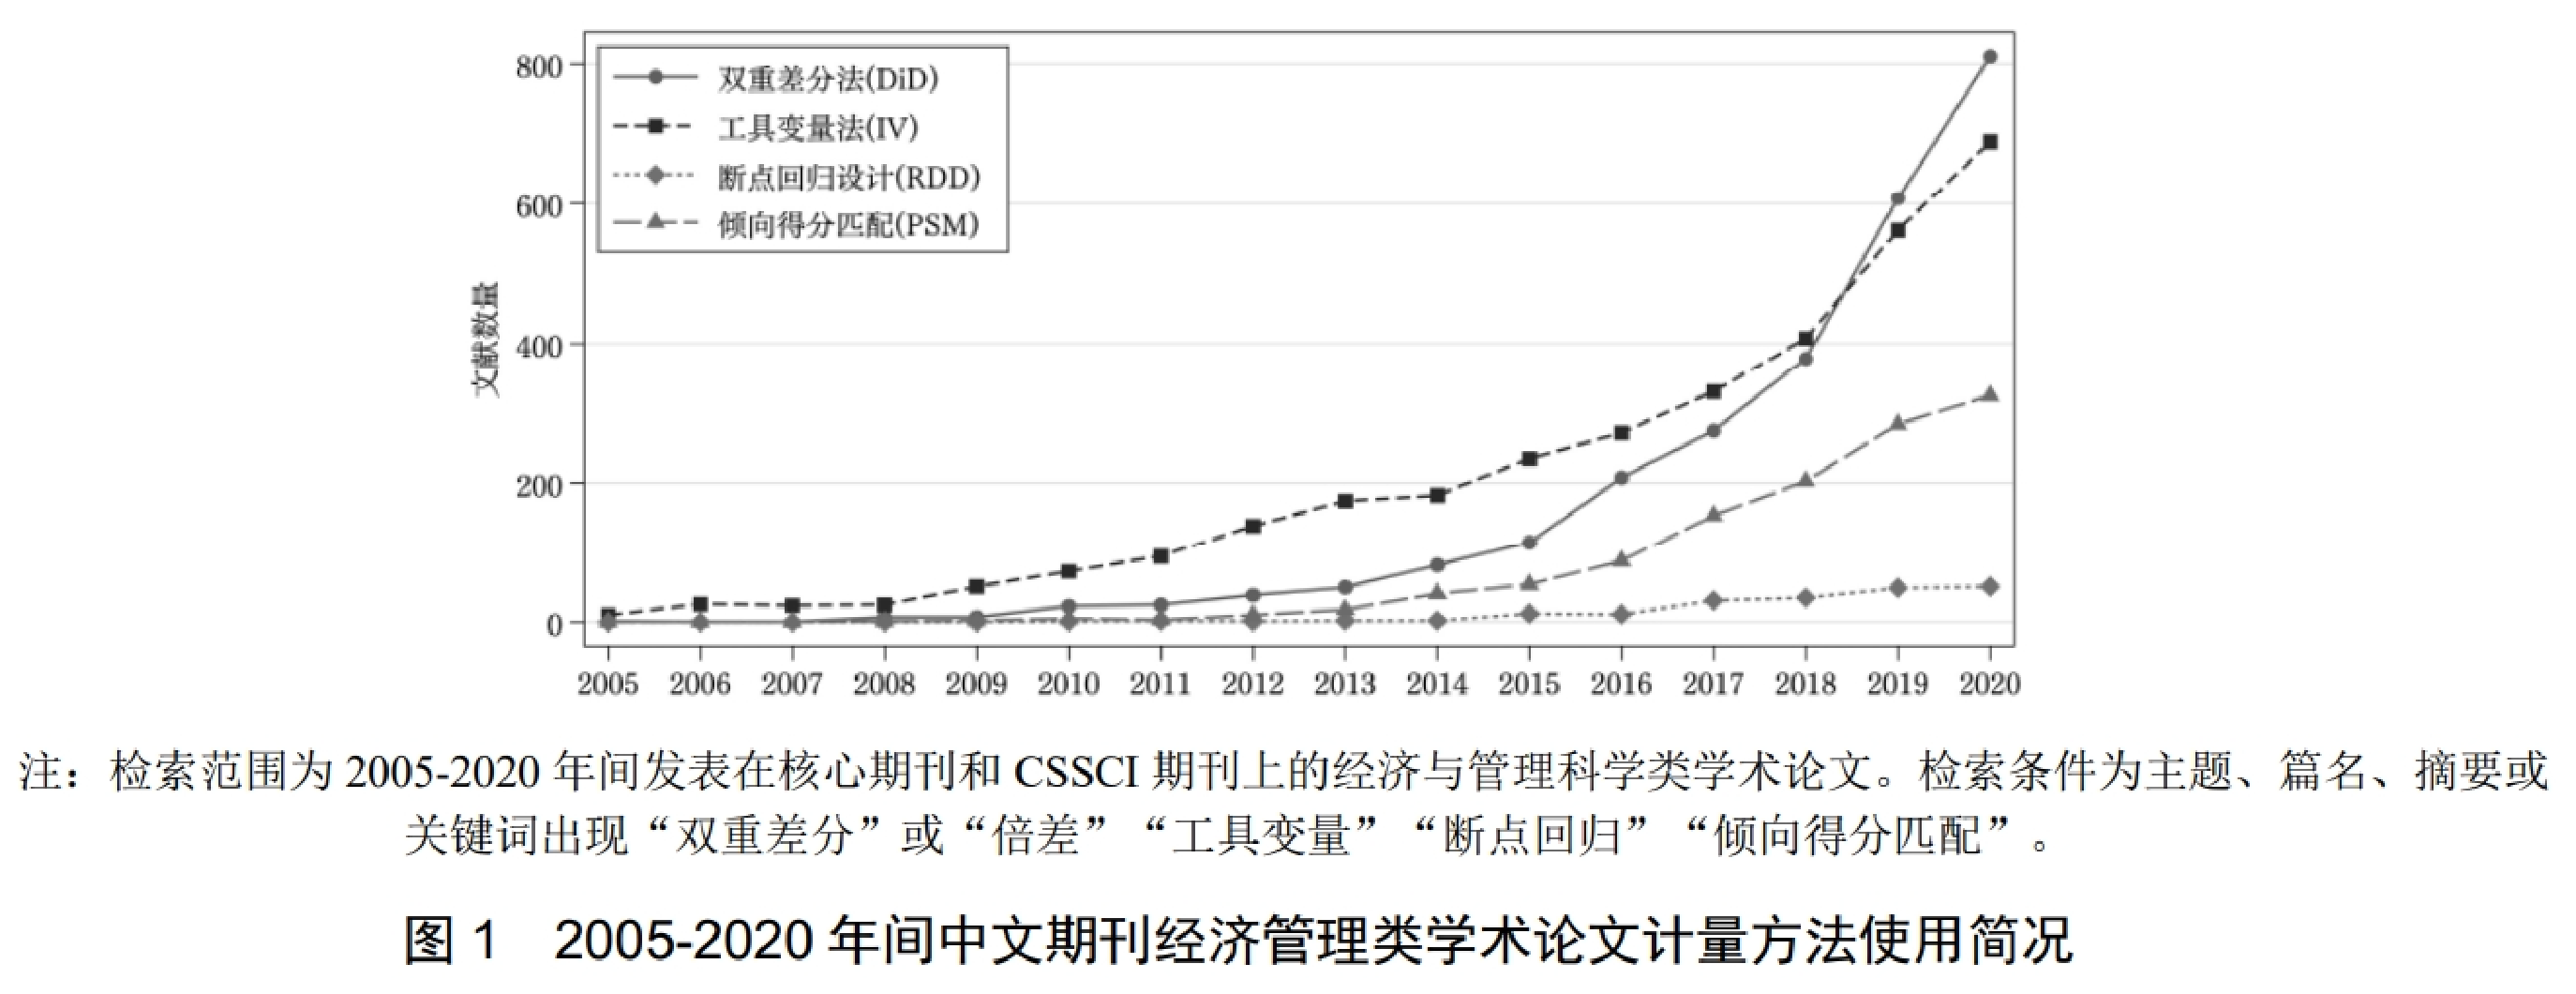
\includegraphics[width=0.9\textwidth]{01}
    \end{figure}
    \begin{center}
        \scriptsize 图片来源:黄炜,张子尧,刘安然.从双重差分法到事件研究法[J].产业经济评论,2022(02):17-36.
    \end{center}
\end{frame}

\begin{frame}
    \begin{itemize}
        \item[$\blacksquare$] 公鸡打鸣与太阳升起
        \item[$\blacksquare$] 夏天的冰淇淋销量与溺水儿童人数
        \item[$\blacksquare$] 刷题与考试成绩
        \item[$\blacksquare$] 受教育年限与毕业工资
    \end{itemize}
\end{frame}

\begin{frame}{双重差分}
    \begin{itemize}
        \item[$\blacksquare$] 双重差分(Difference-in-differences, DID)是计量经济学确定因果关系的常用方法之一
        \item[$\blacksquare$] 比较同一变量在不同时间点或不同地区的值,同时控制其他因素
        \item[$\blacksquare$] 政策评估或对某一外生冲击的评估
        \item[$\blacksquare$] 政策发生时间、受政策影响的样本
    \end{itemize}
\end{frame}


\section{标准DID及其基本原理}

\subsection{双重差分基本思想与Stata实现}

\begin{frame}{标准DID}
    \begin{itemize}
        \item[$\blacksquare$] 统一的政策发生时间、清晰的实验组和对照组
        \item[$\blacksquare$] 设置虚拟变量$T_{i,t}$表示政策发生时间前后
        \item[$\blacksquare$] 设置虚拟变量$D_{i,t}$表示研究样本是否受到政策影响
        \item[$\blacksquare$] 设置估计模型:
    \end{itemize}
    \begin{equation*}
        Y_{i,t}=\beta _0+\beta _1T_{i,t}+\beta _2D_{i,t}+\beta _3T_{i,t}\times D_{i,t}+\varepsilon _{i,t}
    \end{equation*}
\end{frame}

\begin{frame}
    \kaishu
    \begin{equation*}
        Y_{i,t}=\beta _0+\beta _1T_{i,t}+\beta _2D_{i,t}+\alert{\beta _3}T_{i,t}\times D_{i,t}+\varepsilon _{i,t}
    \end{equation*}
    \begin{table}[]
        \begin{tabular}{|ccc|c|}
        \hline
        \multicolumn{1}{|c|}{}                                                          & \multicolumn{1}{c|}{\begin{tabular}[c]{@{}c@{}}政策发生前\\ $T_{i,t}=0$\end{tabular}}  & \begin{tabular}[c]{@{}c@{}}政策发生后\\ $T_{i,t}=1$\end{tabular} & 差分 \\ \hline
        \multicolumn{1}{|c|}{\begin{tabular}[c]{@{}c@{}}实验组\\ $D_{i,t}=1$\end{tabular}} & \multicolumn{1}{c|}{$\beta_0+\beta_1$}                                              & $\beta_0+\beta_1+\beta_2+\beta_3$                             & $\varDelta Y_t=\beta_2+\beta_3$   \\ \hline
        \multicolumn{1}{|c|}{\begin{tabular}[c]{@{}c@{}}对照组\\ $D_{i,t}=0$\end{tabular}} & \multicolumn{1}{c|}{$\beta_0$}                                                      & $\beta_0+\beta_2$                                             & $\varDelta Y_c=\beta_2$   \\ \hline
        \multicolumn{3}{|c|}{Difference in Difference(DID)}                                                                                                                                                                                  & $\varDelta^2 Y=\beta_3$   \\ \hline
        \end{tabular}
    \end{table}
\end{frame}

\begin{frame}
    
\end{frame}

\begin{frame}
    
\end{frame}

\begin{frame}{双重差分核心思想}
    \begin{itemize}
        \item[$\blacksquare$] 双重差分的核心是通过构造交互项来识别政策冲击对受影响个体(实验组)的平均处理效应(Average Treatment effect on the Treated, ATT)
        \item[$\blacksquare$] 在现实中,我们仅能观察到实验组受到冲击后的情况,无法知道实验组如果不受政策冲击的情况
        \item[$\blacksquare$] 双重差分方法将对照组在观察时期内的"变化"近似于实验组倘若未受冲击将发生的变化
    \end{itemize}
\end{frame}

\begin{frame}{标准DID应用}
    \begin{itemize}
        \item[$\blacksquare$] 在实际应用中,双重差分方法经常应用于面板固定数据,此时多采用双向固定效应模型(Two-way fixed effects, TWFE):
        \begin{equation*}
            Y_{i,t}=\alpha+\beta (T_{i,t}\times D_{i,t})+\lambda_t+\mu_i+\varepsilon_{i,t}
        \end{equation*}
        \item[$\blacksquare$] 标准DID中,通常生成政策变量$Policy_{i,t}=T_{i,t}\times D_{i,t}$
    \end{itemize}
\end{frame}

\subsection{平行趋势假设}




\section{渐进DID}

\subsection{美化主题}

\begin{frame}{THU Beamer Theme的新特性}
    \begin{itemize}
        \item 顶栏采用单行圆圈指示
        \item 中文采用楷书
        \item 更多该模板的功能可以参考 \url{https://www.latexstudio.net/archives/4051.html}
        \item 下面列举出了一些Beamer的用法,部分节选自 \url{https://tuna.moe/event/2018/latex/}
    \end{itemize}
\end{frame}

\subsection{如何更好地制作Beamer}

\begin{frame}{Why Beamer}
    \begin{itemize}
        \item \LaTeX 广泛用于学术界,期刊会议论文模板
    \end{itemize}
    \begin{table}[h]
        \centering
        \begin{tabular}{c|c}
            Microsoft\textsuperscript{\textregistered}  Word & \LaTeX \\
            \hline
            文字处理工具 & 专业排版软件 \\
            容易上手,简单直观 & 容易上手 \\
            所见即所得 & 所见即所想,所想即所得 \\
            高级功能不易掌握 & 进阶难,但一般用不到 \\
            处理长文档需要丰富经验 & 和短文档处理基本无异 \\
            花费大量时间调格式 & 无需担心格式,专心作者内容 \\
            公式排版差强人意 & 尤其擅长公式排版 \\
            二进制格式,兼容性差 & 文本文件,易读、稳定 \\
            付费商业许可 & 自由免费使用 \\
        \end{tabular}
    \end{table}
\end{frame}

\begin{frame}{排版举例}
    \begin{exampleblock}{无编号公式} % 加 * 
        \begin{equation*}
            J(\theta) = \mathbb{E}_{\pi_\theta}[G_t] = \sum_{s\in\mathcal{S}} d^\pi (s)V^\pi(s)=\sum_{s\in\mathcal{S}} d^\pi(s)\sum_{a\in\mathcal{A}}\pi_\theta(a|s)Q^\pi(s,a)
        \end{equation*}
    \end{exampleblock}
    \begin{exampleblock}{多行多列公式\footnote{如果公式中有文字出现,请用 $\backslash$mathrm\{\} 或者 $\backslash$text\{\} 包含,不然就会变成 $clip$,在公式里不如 $\mathrm{clip}$ 美观。}}
        % 使用 & 分隔
        \begin{align}
            Q_\mathrm{target}&=r+\gamma Q^\pi(s^\prime, \pi_\theta(s^\prime)+\epsilon)\\
            \epsilon&\sim\mathrm{clip}(\mathcal{N}(0, \sigma), -c, c)\nonumber
        \end{align}
    \end{exampleblock}
\end{frame}

\begin{frame}
    \begin{exampleblock}{编号多行公式}
        % Taken from Mathmode.tex
        \begin{multline}
            A=\lim_{n\rightarrow\infty}\Delta x\left(a^{2}+\left(a^{2}+2a\Delta x+\left(\Delta x\right)^{2}\right)\right.\label{eq:reset}\\
            +\left(a^{2}+2\cdot2a\Delta x+2^{2}\left(\Delta x\right)^{2}\right)\\
            +\left(a^{2}+2\cdot3a\Delta x+3^{2}\left(\Delta x\right)^{2}\right)\\
            +\ldots\\
            \left.+\left(a^{2}+2\cdot(n-1)a\Delta x+(n-1)^{2}\left(\Delta x\right)^{2}\right)\right)\\
            =\frac{1}{3}\left(b^{3}-a^{3}\right)
        \end{multline}
    \end{exampleblock}
\end{frame}

\begin{frame}{图形与分栏}
    \begin{minipage}[c]{0.3\linewidth}
        \psset{unit=0.8cm}
        \begin{pspicture}(-1.75,-3)(3.25,4)
            \psline[linewidth=0.25pt](0,0)(0,4)
            \rput[tl]{0}(0.2,2){$\vec e_z$}
            \rput[tr]{0}(-0.9,1.4){$\vec e$}
            \rput[tl]{0}(2.8,-1.1){$\vec C_{ptm{ext}}$}
            \rput[br]{0}(-0.3,2.1){$\theta$}
            \rput{25}(0,0){%
            \psframe[fillstyle=solid,fillcolor=lightgray,linewidth=.8pt](-0.1,-3.2)(0.1,0)}
            \rput{25}(0,0){%
            \psellipse[fillstyle=solid,fillcolor=yellow,linewidth=3pt](0,0)(1.5,0.5)}
            \rput{25}(0,0){%
            \psframe[fillstyle=solid,fillcolor=lightgray,linewidth=.8pt](-0.1,0)(0.1,3.2)}
            \rput{25}(0,0){\psline[linecolor=red,linewidth=1.5pt]{->}(0,0)(0.,2)}
%           \psRotation{0}(0,3.5){$\dot\phi$}
%           \psRotation{25}(-1.2,2.6){$\dot\psi$}
            \psline[linecolor=red,linewidth=1.25pt]{->}(0,0)(0,2)
            \psline[linecolor=red,linewidth=1.25pt]{->}(0,0)(3,-1)
            \psline[linecolor=red,linewidth=1.25pt]{->}(0,0)(2.85,-0.95)
            \psarc{->}{2.1}{90}{112.5}
            \rput[bl](.1,.01){C}
        \end{pspicture}
    \end{minipage}\hspace{1cm}
    \begin{minipage}{0.5\linewidth}
        \medskip
        %\hspace{2cm}
        \begin{figure}[h]
            \centering
            \includegraphics[height=.4\textheight]{pic/dtmf.pdf}
        \end{figure}
    \end{minipage}
\end{frame}

\begin{frame}[fragile]{\LaTeX{} 常用命令}
    \begin{exampleblock}{命令}
        \centering
        \footnotesize
        \begin{tabular}{llll}
            \cmd{chapter} & \cmd{section} & \cmd{subsection} & \cmd{paragraph} \\
            章 & 节 & 小节 & 带题头段落 \\\hline
            \cmd{centering} & \cmd{emph} & \cmd{verb} & \cmd{url} \\
            居中对齐 & 强调 & 原样输出 & 超链接 \\\hline
            \cmd{footnote} & \cmd{item} & \cmd{caption} & \cmd{includegraphics} \\
            脚注 & 列表条目 & 标题 & 插入图片 \\\hline
            \cmd{label} & \cmd{cite} & \cmd{ref} \\
            标号 & 引用参考文献 & 引用图表公式等\\\hline
        \end{tabular}
    \end{exampleblock}
    \begin{exampleblock}{环境}
        \centering
        \footnotesize
        \begin{tabular}{lll}
            \env{table} & \env{figure} & \env{equation}\\
            表格 & 图片 & 公式 \\\hline
            \env{itemize} & \env{enumerate} & \env{description}\\
            无编号列表 & 编号列表 & 描述 \\\hline
        \end{tabular}
    \end{exampleblock}
\end{frame}

\begin{frame}[fragile]{\LaTeX{} 环境命令举例}
    \begin{minipage}{0.5\linewidth}
\begin{lstlisting}[language=TeX]
\begin{itemize}
  \item A \item B
  \item C
  \begin{itemize}
    \item C-1
  \end{itemize}
\end{itemize}
\end{lstlisting}
    \end{minipage}\hspace{1cm}
    \begin{minipage}{0.3\linewidth}
        \begin{itemize}
            \item A
            \item B
            \item C
            \begin{itemize}
                \item C-1
            \end{itemize}
        \end{itemize}
    \end{minipage}
    \medskip
    \pause
    \begin{minipage}{0.5\linewidth}
\begin{lstlisting}[language=TeX]
\begin{enumerate}
  \item 一级 \item 二级
  \item 三级
  \begin{itemize}
    \item[a.] 子标题
  \end{itemize}
\end{enumerate}
\end{lstlisting}
    \end{minipage}\hspace{1cm}
    \begin{minipage}{0.3\linewidth}
        \begin{enumerate}
            \item 一级
            \item 二级
            \item 三级
            \begin{itemize}
                \item[a.] 子标题
            \end{itemize}
        \end{enumerate}
    \end{minipage}
\end{frame}

\begin{frame}[fragile]{\LaTeX{} 数学公式}
    \begin{columns}
        \begin{column}{.55\textwidth}
\begin{lstlisting}[language=TeX]
$V = \frac{4}{3}\pi r^3$

\[
  V = \frac{4}{3}\pi r^3
\]

\begin{equation}
  \label{eq:vsphere}
  V = \frac{4}{3}\pi r^3
\end{equation}
\end{lstlisting}
        \end{column}
        \begin{column}{.4\textwidth}
            $V = \frac{4}{3}\pi r^3$
            \[
                V = \frac{4}{3}\pi r^3
            \]
            \begin{equation}
                \label{eq:vsphere}
                V = \frac{4}{3}\pi r^3
            \end{equation}
        \end{column}
    \end{columns}
    \begin{itemize}
        \item 更多内容请看 \href{https://zh.wikipedia.org/wiki/Help:数学公式}{\color{purple}{这里}}
    \end{itemize}
\end{frame}

\begin{frame}[fragile]
    \begin{columns}
        \column{.6\textwidth}
\begin{lstlisting}[language=TeX]
    \begin{table}[htbp]
      \caption{编号与含义}
      \label{tab:number}
      \centering
      \begin{tabular}{cl}
        \toprule
        编号 & 含义 \\
        \midrule
        1 & 4.0 \\
        2 & 3.7 \\
        \bottomrule
      \end{tabular}
    \end{table}
    公式~(\ref{eq:vsphere}) 的
    编号与含义请参见
    表~\ref{tab:number}。
\end{lstlisting}
        \column{.4\textwidth}
        \begin{table}[htpb]
            \centering
            \caption{编号与含义}
            \label{tab:number}
            \begin{tabular}{cl}\toprule
                编号 & 含义 \\\midrule
                1 & 4.0\\
                2 & 3.7\\\bottomrule
            \end{tabular}
        \end{table}
        \normalsize 公式~(\ref{eq:vsphere})的编号与含义请参见表~\ref{tab:number}。
    \end{columns}
\end{frame}

\begin{frame}{作图}
    \begin{itemize}
        \item 矢量图 eps, ps, pdf
        \begin{itemize}
            \item METAPOST, pstricks, pgf $\ldots$
            \item Xfig, Dia, Visio, Inkscape $\ldots$
            \item Matlab / Excel 等保存为 pdf
        \end{itemize}
        \item 标量图 png, jpg, tiff $\ldots$
        \begin{itemize}
            \item 提高清晰度,避免发虚
            \item 应尽量避免使用
        \end{itemize}
    \end{itemize}
\end{frame}

\section{其他DID拓展}
\begin{frame}
    \begin{itemize}
        \item 一月:文献调研
        \item 二月:Beamer主题复现、美观程度评测
        \item 三、四月:Beamer主题美化
        \item 五月:论文撰写
    \end{itemize}
\end{frame}

\section{DID论文结构与参考文献}

\begin{frame}[allowframebreaks]
    \bibliography{ref}
    \bibliographystyle{alpha}
    % 如参考文献较多,可按如下方式调整字体:
    % \tiny\bibliographystyle{alpha}
\end{frame}

\begin{frame}
    \begin{center}
        {\Huge\calligra Thanks!}
    \end{center}
\end{frame}

\end{document}